% !TeX spellcheck = hu_HU
% !TeX encoding = UTF-8
\chapter{Teljesítménymérési keretrendszer}\label{sec:keretrendszer}

A gráfalapú és a relációs adatbázis-kezelők teljesítményének és a használhatóságának összehasonlítása az adatbázis-kezelők fejleszőinek és a felhasználóinak is fontos információk forrása lehet. A fejlesztők megtudhatják, hogy a rendszerük mennyire hatékony a többi adatbázis-kezelőhöz képes, a felhasználók pedig a mérési eredmények révén több információ alapján választhatják ki a számukra megfelelő adatbázis-kezelőt.

A különböző adatbázisok és nyelvek összehasonlítása során szükség volt egy teljesítménymérési keretrendszerre, amely fókuszában a gráfadatbázisok állnak. Kiemelt szempont volt, hogy a keretrendszer lekérdezései általános formában legyenek definiálva, ne pedig egy adott lekérdezési nyelven megírt lekérdezésekkel. Ezen feltétel alapján a Linked Data Benchmark Council (LDBC)\footnote{A szervezet honlapja: \url{http://ldbcouncil.org}} szervezet Social Network Benchmark (SNB) keretrendszerét választottam, mert ez az elérhető legátfogóbb teljesítménymérési keretrendszer gráf információs rendszerek összehasonlító teljesítménymérésére.

Az LDBC egy európai uniós projekt keretében létrejött szervezet, amelynek célja teljesítménymérési keretrendszerek, munkafolyamatok létrehozása gráf vagy RDF alapú adatbázis-kezelő rendszerekhez, valamint az auditált mérési eredmények publikálása. Jelenleg több nagy cég támogatja a szervezetet\footnote{Az aktuális partnercégek listája megtekinthető a szervezet honlapján: \url{http://ldbcouncil.org/industry/members}}, mint például az Oracle, IBM, Intel, Neo4j és OpenLink Software (a Virtuoso gyártója).

\section{LDBC Social Network Benchmark}

Az LDBC SNB célja a gráf típusú adatbázis-kezelő rendszerek funkciójának széles körű tesztelése. Ehhez a keretrendszer egy szintetikus közösségi háló gráf alapú adatbázisát használja. Az adathalmaz sémája \aref{fig:dataschema}.~ábrán látható. A keretrendszer kétféle terhelési profilt tartalmaz.

Az úgynevezett \textit{Business Intelligence}~\cite{DBLP:conf/sigmod/ErlingALCGPPB15} (BI) terhelési profil olyan analitikus lekérdezéseket fogalmaz meg, amelyeknek a megválaszolásához az adathalmaz átfogó vizsgálata szükséges, például minden felhasználó üzeneteinek megszámolása. Ilyen lekérdezés például a legaktívabb, vagy éppen a legkevésbé aktív felhasználók megkeresése, vagy a baráti háromszögek megkeresése. A terhelési profil tervezése során gondosan figyeltek az olyan különböző kihívásokra, amelyeket az adatbázis-kezelő rendszereknek hatékonyan kell kezelni ahhoz, hogy nagyméretű adathalmazokon is megfelelő teljesítményt nyújtsanak. Ezek a kihívások a funkcionalitás széles köréből gyűjtötték össze: a relációs adatbázis-kezelőknél megfigyelt nehézségeken túl többek között a lekérdezőnyelvek kifejezőerejét, vagy a gráf specifikus lekérdezések komplexitását is vizsgálták ezen szempontrendszer felépítéséhez. A két teljesítménymérési profil közül a BI jött létre később, véglegesítése még jelenleg is folyamatban van.

Az \textit{Interactive}~\cite{DBLP:conf/grades/SzarnyasPAMPKEB18} profil lekérdezései pedig inkább egy, vagy néhány csomóponthoz kapcsolódó adat alapos vizsgálatát követelik meg. Az \textit{Interactive} profil lekérdezései három további csoportba sorolhatóak: 
\begin{itemize}
	\item Komplex lekérdezések (Complex reads, CR), 14 darab: Az adathalmaz számos pontját, általában egy ember ismerőseit és azok ismerőseit, valamint az ő aktivitásukat érintő lekérdezések. 
	\item Rövid lekérdezések (Short reads, SR), 7 darab: Egyszerű, általában öt csomópontnál nem többet érintő lekérdezések.
	\item Frissítések (Updates, U), 8 darab: Legfejlebb egy csomópont és néhány él beszúrása az adathalmazba.
\end{itemize}
A két terhelési profil két fontos tulajdonságának összehasonlítását mutatja \aref{fig:ldbc-graph-benchmarks}.~ábra: a feltételezett válaszidőt és a lekérdezés során megvizsgált adatmennyiséget. 
\begin{figure}[htb]
	\centering
	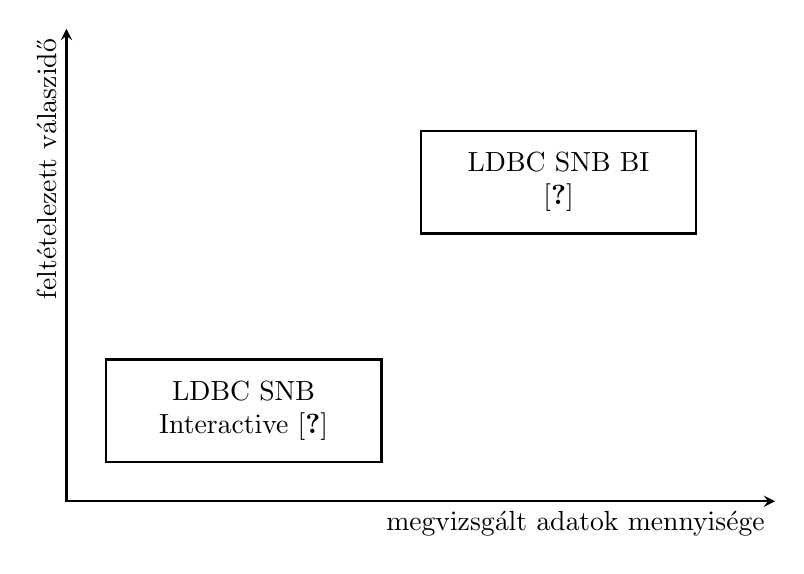
\begin{tikzpicture}[scale=1,thick]
	\tikzstyle{every node} = [align=center]
	
	\draw [stealth-stealth]
	(0,6.0) node (yaxis) [above left,rotate=90] {feltételezett válaszidő}
	|- (9.0,0) node (xaxis) [below left] {megvizsgált adatok mennyisége};
	
	\draw (0.5,0.5) rectangle ++(3.5,1.3) node[pos=0.5,text width=4cm] {LDBC SNB \\ Interactive \cite{DBLP:conf/sigmod/ErlingALCGPPB15}};
	\draw (4.5,3.4) rectangle ++(3.5,1.3) node[pos=0.5,text width=4cm] {LDBC SNB BI \\ \cite{DBLP:conf/grades/SzarnyasPAMPKEB18}};
	\end{tikzpicture}
	\caption{A teljesítménymérési profilok karakterisztikája.}
	\label{fig:ldbc-graph-benchmarks}
\end{figure}

Ahhoz, hogy a különböző rendszerek teljesítményét átfogóan lehessen elemezni, a keretrendszer támogatja az adathalmaz skálázását is. Az adathalmaz skálázási együtthatóját (scale factor, SF) a CSV\footnote{Comma-Separated Values} formátumban tárolt adathalmaz gigabájtban számolt mérete adja. A keretrendszer által előre konfigurált skálázási együtthatók a következők: 0.1, 0.3, 3, 10, 30, 100, 300, 1000. A különböző skálázási együtthatójú adathalmazok méretének szabályozása az adathalmazban szereplő emberek számának megadásával történik, ennek megfelelően generálódik a hálózat többi része. A mérésekhez használt SF1-es adathalmazban 11 ezer, az SF3-asban 27 ezer, az SF10-esben 73 ezer ember szerepel~\cite{LDBC_SNB}.

Az LDBC SNB lekérdezéseinek specifikációja tartalmaz egy szemléltető ábrát, és a lekérdezés szabadszöveges megfogalmazását is. Ennek köszönhetően nem csak az adatbázis-kezelő rendszerek, de a lekérdezési nyelvek összehasonlítására is alkalmas a keretrendszer.

\subsection{A teljesítménymérés munkafolyamata}

A keretrendszer munkafolyamatát \aref{fig:workflow}.~ábra mutatja be. A munkafolyamatban négy típusú összetevő van: \textit{(1)} a keretrendszerhez kapcsolódó szoftvermodulok és a lekérdezések forráskódja, \textit{(2)} eljárás, \textit{(3)} emberek által definiált adat és \textit{(4)} generált adat. Az összetevőket továbbá két csoportba sorolhatjuk az alapján, hogy az elkészítésük vagy végrehajtásuk a keretrendszer fejlesztőinek (LDBC SNB munkacsoport) vagy felhasználóinak (Adatbázis-kezelők fejlesztői, felhasználói) a feladata.

A keretrendszer fejlesztőinek feladatai:
\begin{itemize}
	\item A \textit{lekérdezések specifikációnak}\footnote{\url{https://github.com/ldbc/ldbc_snb_docs}} elkészítése és karbantartása~\cite{LDBC_SNB}
	\item Az adathalmazokat és lekérdezések paramétereit \textit{generáló alkalmazás} (DATAGEN)\footnote{\url{https://github.com/ldbc/ldbc_snb_datagen}} elkészítése
	\item A megvalósítások ellenőrzése és a teljesítménymérést végző \textit{alkalmazás keretrendszer} (DRIVER)\footnote{\url{https://github.com/ldbc/ldbc_snb_driver}} elkészítése
	\item A \textit{referenciaimplementáció} elkészítése
	\item Az egyes lekérdezések elvárt eredményét tartalmazó adathalmaz, azaz a \textit{referencia validációs adathalmaz} elkészítése
\end{itemize}
Ezen részfolyamatok elkészülte után a felhasználók elkezdhetik megvalósítani a saját összetevőket. A DATAGEN modullal a felhasználók generálhatnak adott méretű adathalmazt, illetve a hozzá tartozó lekérdezés paramétereket. A dolgozat készítése során a Sparksee implementációt tekintettem referenciaimplementációnak.

A felhasználók által végzett munkát további két csoportba lehet osztani: az implementáció ellenőrzése és a teljesítménymérés. Mindkettőhöz szükséges az adott adatbázis-kezelőhöz tartozó szoftvermodulok és lekérdezések implementációja. A szoftvermodulok közé tartoznak az adatok betöltését, a lekérdezések futtatását végző és az eredményeket a DRIVER számára feldolgozható formátumra konvertáló modulok. Az ellenőrzés lépései ezek után az alábbiak:
\begin{itemize}
	\item Az \textit{ellenőrzési beállítások} (például mennyi lekérdezést futtason a keretrendszer) és a \textit{lekérdezés paraméterek} alapján az \textit{eszközhöz tartozó validációs adatok} (a lekérdezések eredményeinek) előállítása
	\item Az eredmények összevetése a referencia validációs adathalmazzal: ha az eredmény megegyezik a referencia validációs adathalmazzal, akkor következhet a teljesítménymérés, ellenkező esetben a hibákat javítani kell és újra ellenőrizni az implementációt
\end{itemize}
A felhasználói beállítások sok finomhangolási lehetőséget biztosítanak, például mennyi végrehajtási szálon fusson egyidőben az ellenőrzés, összesen mennyi lekérdezést végezzen el, illetve az egyes lekérdezések ellenőrzését egyenként lehet engedélyezni vagy tiltani, stb..

\begin{figure}[h]
	\centering
	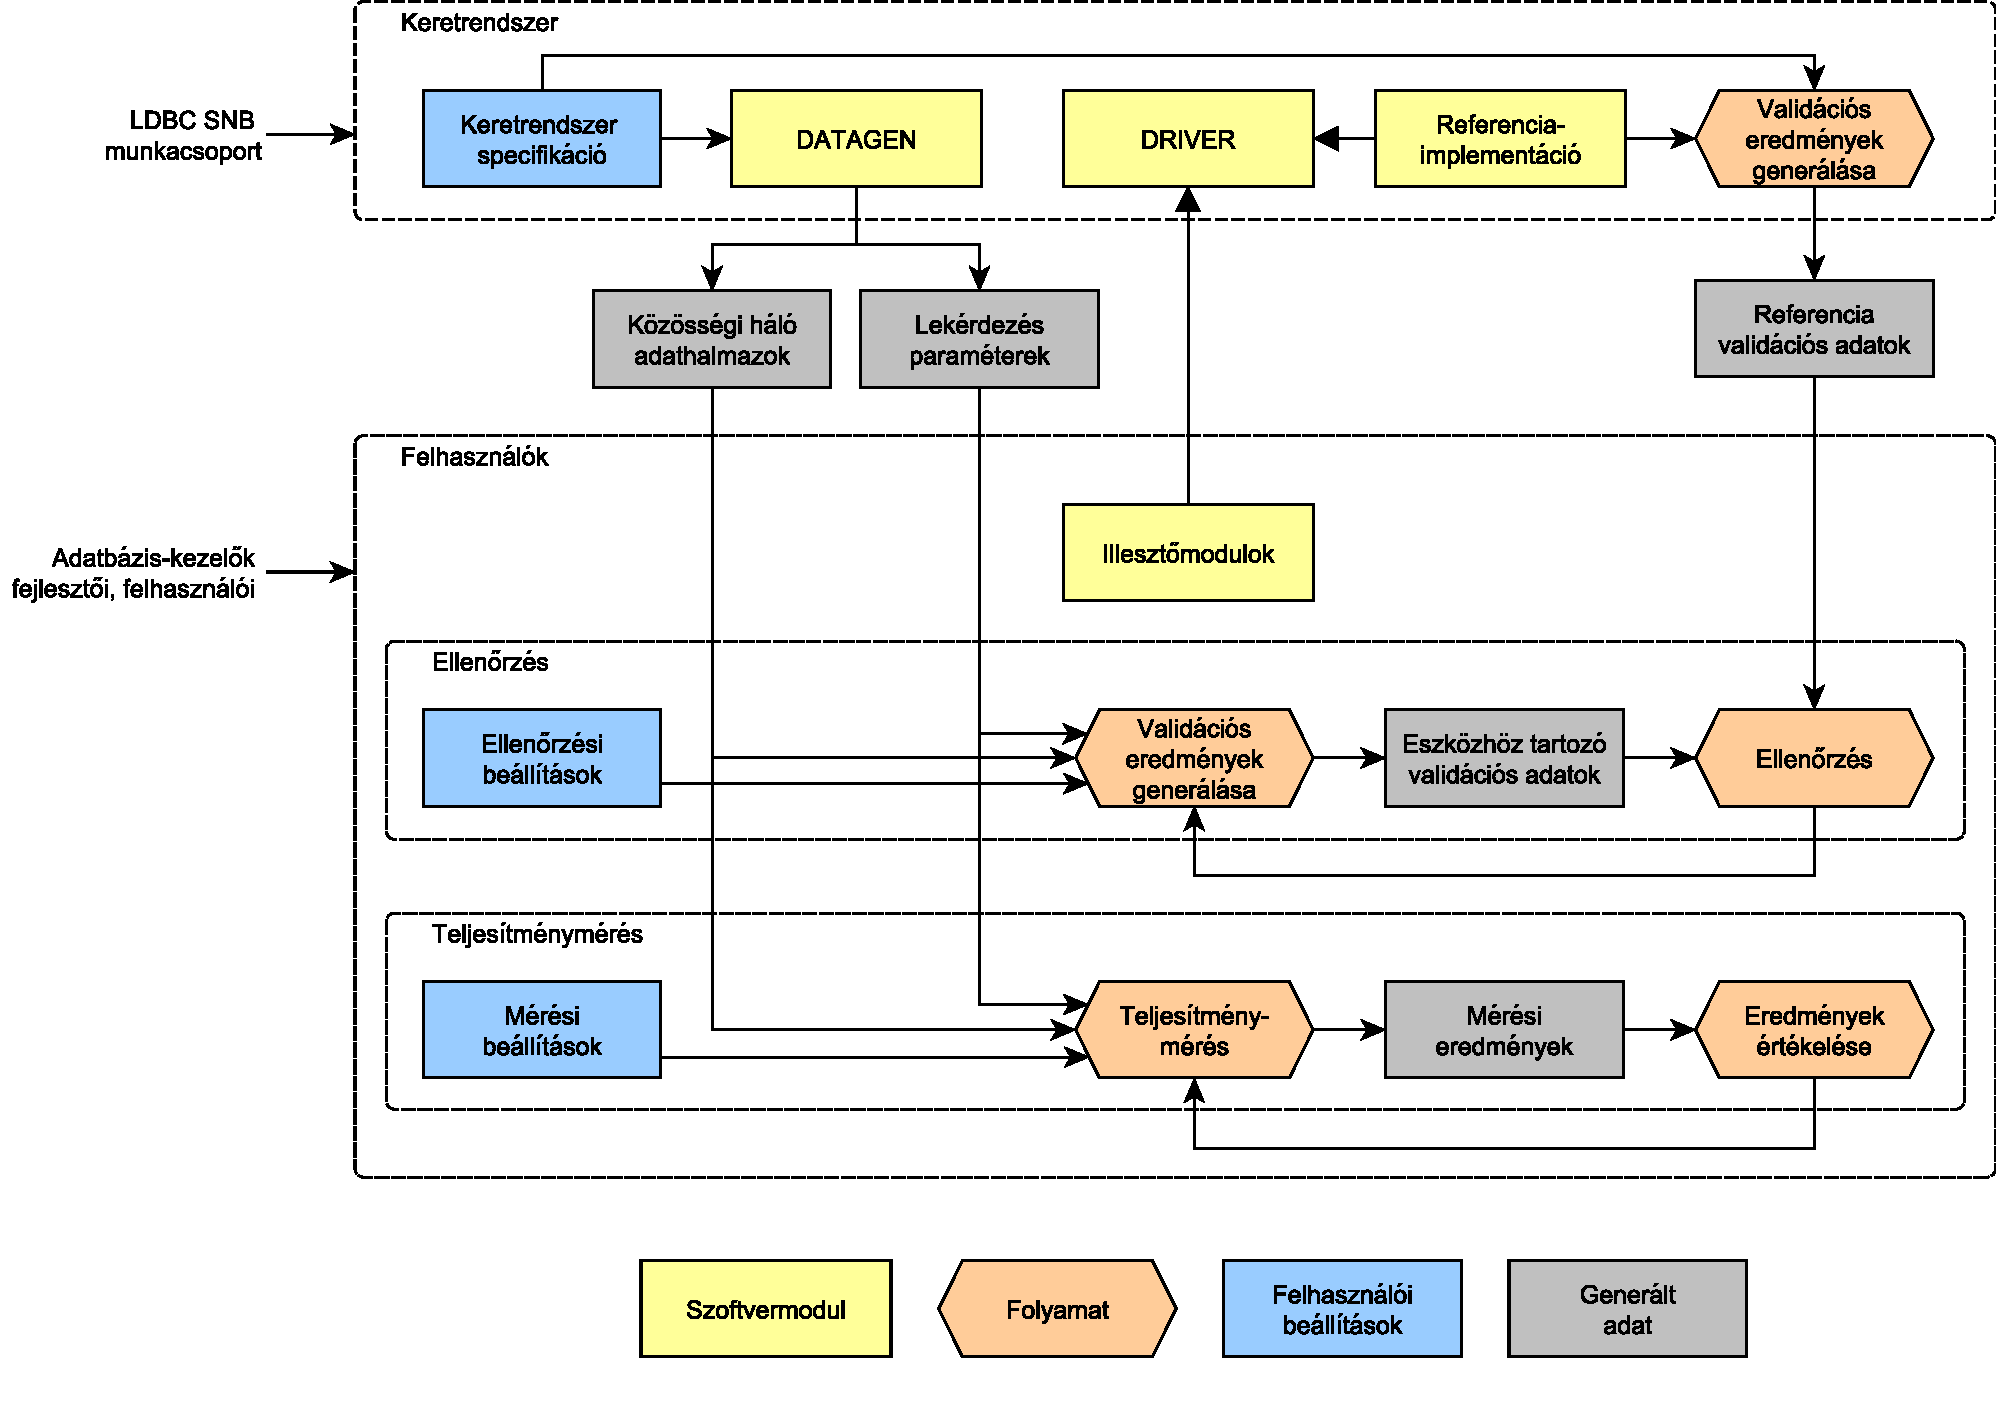
\includegraphics[width=\linewidth]{workflow.pdf}
	\caption{A teljesítménymérési keretrendszer munkafolyamata}
	\label{fig:workflow}
\end{figure}

Ha az implementáció átment az ellenőrzésen, akkor a teljesítménymérés a következő lépés. A teljesítménymérés lépései hasonlóak az ellenőrzés lépéseihez:
\begin{itemize}
	\item A \textit{mérési beállítások} és a lekérdezés paraméterek alapján a teljesítményérés futtatásával a \textit{mérési eredmények} elkészítése
	\item Az eredmények értékelése és esetleges új mérés indítása (például nagyobb méretű adathalmazon)
\end{itemize}

\section{Teljesítménymérési keretrendszer bővítése}
A dolgozat készítése során az LDBC SNB-t bővítettem a \textit{Business Intelligence} terhelési profil SPARQL, és az \textit{Interactive} terhelési profil SPARQL és Cypher implementációjával, ezzel bővítve ki a keretrendszerrel lemérhető adatbázis-kezelők halmazát. Ezen felül implementáltam egy Gremlin-t támogató adatbázis-kezelőkhöz használható adatbetöltő alkalmazást.
\subsection{Business Intelligence terhelési profil}

A Business Intelligence terhelési profil lekérdezéseit SPARQL nyelven készítettem el. A lekérdezéseknek nem létezett SPARQL megvalósítása. A lekérdezések komplexitásából adódóan az implementálás során sok esetben a nyelv kifejezőerejét is próbára tették. A 25-ös lekérdezést nem is lehet szabványos SPARQL-ben megvalósítani, mert nem támogatja a legrövidebb utak keresését. A következőkben bemutatom az általam legérdekesebb, vagy legnagyobb kihívásokat, amelyekkel az implementáció készítése során szembesültem.

\paragraph{NULL érték kezelése}
A megszokott lekérdezési nyelvekkel ellentétben a SPARQL-ben nincsenek a megszokott értelemben vett NULL értékek: a változók lehetnek kötöttek, vagy kötetlenek, azaz vagy tartozik hozzájuk egy érték vagy nem. Az egyszerű gráfminták csak akkor illeszkednek egy adott részgráfra, ha minden változó kötött, azaz mindegyikhez tartozik egy érték. Ez alól az egyetlen kivétel a \keyword{OPTIONAL} kulcsszóval megadott opcionális gráfminták, mert az azokban megadott változók lehetnek kötetlenek. Fontos megjegyezni, hogy egy opcionális gráfmintában megadott változókat tekintve vagy mind kötött, vagy egyik sem, azaz az ilyen minták esetében is igaz az, hogy csak akkor illeszkednek, ha minden változójuk kötött. Például a \listref{sparql-null}~kódrészletben szereplő SPARQL lekérdezés eredményében az \textit{?a}, \textit{?b} és \textit{?c} változók mindig kötöttek lesznek, míg a \textit{?i} és \textit{?j} közül vagy mindkettő kötött, vagy mindkettő kötetlen lesz az eredmény egy sorában.

\vspace{1.5ex}

\noindent\begin{minipage}{\textwidth}
\begin{lstlisting}[frame=single, morekeywords={SELECT},label=listing:sparql-null, caption=Példa az OPTIONAL kulcsszóra]
SELECT
	?a, ?b, ?c, ?i, ?j
WHERE
{
	?a predicate1 ?b .
	?b predicate2 ?c .
	OPTIONAL {
		?a predicate3 ?i .
		?b predicate4 ?j 
	}
}
\end{lstlisting}
\end{minipage}

\paragraph{Nevesített gráfminták hiánya}
A SPARQL nem támogatja nevesített gráfminták létrehozását, így nem lehet többször felhasználható gráfmintákat létrehozni. Ez kifejezetten kényelmetlenné teszi a 15-öshöz hasonló lekérdezések leírását. A 15-ös lekérdezés grafikus specifikációja látható a \figref{bi15}~ábrán. Jól látható, hogy az azonos országból származó barátok megszámolására kétszer is szükség van, azonban mivel a gráfmintát nem lehet elnevezni, így a lekérdezésben is kétszer kellett leírni ugyanazt a gráfmintát. Összetett gráfmintáknál a több példány szinkronban tartása kényelmetlen és sok hibalehetőséget hordoz.

\begin{figure}[!ht]
	\centering
	\includegraphics[width=\textwidth, keepaspectratio]{bi-read-15}
	\caption[]{A BI15-ös lekérdezés}
	\label{fig:bi15}
\end{figure}

\paragraph{Deklarációk hiánya}
Mivel SPARQL nyelvben a változók deklarálása a változóra történő első hivatkozás, így a hosszabb lekérdezések esetében az esetleges elgépelésekkel újabb, természetesen nem kívánt változókat deklarálhatunk. Ezen a nyelv megváltoztatása nélkül egy megfelelő SPARQL szerkesztővel lehet segíteni, azonban a dolgozat készítése közben nem sikerült ilyen eszközt találni, a SPARQL szintaxis kiemelését is csak néhány egyszerű szöveges szerkesztő támogatja. A deklarációk hiánya egyébként több másik lekérdezőnyelvben is problémát jelent (pl. Datalog, Cypher, VQL).

\paragraph{Utak hosszának definiálása}
Bár SPARQL-ben van lehetőség változó hosszú útvonal-kifejezések leírására, azonban a Cypher \lstinline{x..y} alakú kifejezésével megegyező nyelvi konstrukciót nem tartalmaz a SPARQL. Ez a nyelvi konstrukció azonban szükséges a \figref{bi16}~ábrán látható 16-os lekérdezés megvalósításához, mivel a benne lévő út hossza a lekérdezése paramétere. Ennek ellenére a 16-os lekérdezéshez készítettem egy olyan implementációt, amelyben az útvonal-kifejezést a keretrendszer szoftvermodulja generálja le és illeszti be a SPARQL lekérdezésbe, így megteremtve a lehetőségét a nem triviális útvonal-kifejezéseket tartalmazó lekérdezések összehasonlítására.

\begin{figure}[!ht]
	\centering
	\includegraphics[width=\textwidth, keepaspectratio]{bi-read-16}
	\caption[]{A BI16-os lekérdezés}
	\label{fig:bi16}
\end{figure}

\subsection{Interactive terhelési profil}
\subsubsection{SPARQL implementációk}

Az interaktív terhelési profil CR és SR lekérdezéseinek két implementációja (az egyik az LDBC SNB implementációja, a másik pedig egy szabadon elérhető implementáció\footnote{A Waterloo-i Egyetemen fejlesztett implementáció: \url{https://github.com/anilpacaci/ldbc_snb_implementations}}~\cite{DBLP:conf/grades/PacaciZLO17}) is létezett, de több probléma is volt velük:
\begin{itemize}
	\item A lekérdezések csak a Virtuoso adatbázis saját SPARQL dialekutásban voltak elérhetők. A Virtuoso SPARQL dialektusa több olyan konstrukciót tartalmaz, ami az eredeti SPARQL nyelvhez képest tömörebb és kifejezőbb lekérdezések írását teszi lehetővé. Ezek átírása szabványos SPARQL nyelvre nem-triviális lépéseket igényel, és nem is lehetséges minden esetben.
	\item A lekérdezések specifikációi az implementáció elkészülte óta pontosítva, javítva lettek, így néhány lekérdezés hibássá vált.
	\item Néhány lekérdezés nem a leghatékonyabb struktúrájú volt.
\end{itemize}
Ezen okok miatt a lekérdezések teljes újraimplementálása mellett döntöttem, nem próbáltam meg a meglévő lekérdezéseket átalakítani. A munka során a specifikáció alapján implementáltam\footnote{SPARQL implementáció: \url{https://github.com/ldbc/ldbc_snb_implementations/pull/51}} 27 darab (12 db CR, 7 db SR, 8 db U) lekérdezést SPARQL nyelven.

A CR13 lekérdezéshez szükséges egy legrövidebb út megtalálása, a CR14 lekérdezéshez az összes legrövidebb út megtalálása és súlyozása az érintett csomópontok alapján. Ezeket a funkciókat a SPARQL szabvány nem tartalmazza, így ezeket a lekérdezéseket nem implementáltam. Az implementáció elkészítése során \textit{(1)} implementáltam a 27 darab lekérdezést SPARQL nyelven, \textit{(2)} implementáltam a lekérdezések végrehajtását és a lekérdezések eredményének konvertálását végző szoftvermodulokat Java nyelven, \textit{(3)} a keretrendszert használva sikeresen végrehajtottam az implementáció ellenőrzését.

A munkát nehezítette, hogy a lekérdezések specifikációi sok esetben pontosításra, vagy kiegészítésre szorultak, vagy az adathalmaz régebbi változtatásai miatt frissíteni kellett azokat. Tehát a terhelési profil lekérdezéseinek implementálása közben a terhelési profilhoz kapcsolódó dokumentációkat is frissítettem, kiegészítettem, így megkönnyítve más felhasználóknak a saját lekérdezéseik és moduljaik elkészítését.

\subsubsection{Cypher implementációk}

A terhelési profilhoz nem volt elkészítve a Cypher implementáció, azonban egy másik nyílt forráskódú projektben\footnote{A Stanford Egyetemen fejlesztett implementáció: \url{https://github.com/PlatformLab/ldbc-snb-impls}} a lekérdezések jelentős része implementálásra került. Bár ezek a lekérdezések sem voltak hibátlanok, minőségük jelentősen jobb volt, mint a SPARQL-ben létező lekérdezéseké, így ezeket fel tudtam használni a végleges implementáció\footnote{Cypher implementáció: \url{https://github.com/ldbc/ldbc_snb_implementations/pull/57}} elkészítéséhez. A SPARQL implementációhoz hasonló módon itt is három részre lehet osztani az elvégzett munkát: \textit{(1)} a meglévő lekérdezések implementációjának ellenőrzése és javítása, illetve a hiányzók implementálása Cypher nyelven, \textit{(2)} a szükséges szoftvermodulok implementációja, \textit{(3)} az implementáció ellenőrzése. Fontos megjegyezni, hogy a jelenleg szabványosítás alatt álló openCypher nyelv nem tartalmazza a legrövidebb utak kifejezésére szolgáló nyelvi konstrukciókat (pl. \texttt{shortestPath} és \texttt{allShortestPath}), így CR13 és CR14 lekérdezések csak Cypher (és nem openCypher) nyelven értelmezhetőek.

\subsubsection{Gremlin adatbetöltő}
A dolgozat készítése során megpróbálkoztam a Cypher for Gremlin\footnote{\url{https://github.com/opencypher/cypher-for-gremlin}} projekt felhasználásával a keretrendszert kiterjeszteni a Gremlin-t támogató adatbázis-kezelőkre is, azonban nem sikerült minden technikai problémát megoldani a dolgozat elkészültéig. Még a triviális Cypher lekérdezésekből generált Gremlin lekérdezések is igen nagy méretűek, a generált jellegből fakadóan az elnevezések nem intuitívak, így a lekérdezések futtatása, a hibakeresés vagy éppen az eredmények megfelelő formátumra való konvertálása sem triviális feladat. \listref{cypher-example}~kódrészletben szereplő Cypher lekérdezésből az alábbi Gremlin lekérdezést állítja elő a projekt:
\begin{lstlisting}[frame=single,language=Java]
g.V().as('p').hasLabel('Person').as('p').choose(__.select('p').is(neq('  cypher.null')).outE('KNOWS').inV().as('f').hasLabel('Person'), __.select('p').is(neq('  cypher.null')).outE('KNOWS').inV().as('f').hasLabel('Person'), __.constant('  cypher.null').as('f')).select('p', 'f').group().by(__.select('p').choose(neq('  cypher.null'), __.choose(__.values('name'), __.values('name'), __.constant('  cypher.null')), __.constant('  cypher.null'))).by(__.fold().project('p.name', 'count(f)').by(__.unfold().select('p').choose(neq('  cypher.null'), __.choose(__.values('name'), __.values('name'), __.constant('  cypher.null')), __.constant('  cypher.null'))).by(__.unfold().select('f').is(neq('  cypher.null')).count())).unfold().select(values)
\end{lstlisting}
Az implementáció nem teljes körű, de az adatok betöltését végző szoftvermodul funkcionalitását tekintve elkészült, az adatok betöltésére alkalmas.
